\chapter{Molecular Aggregates and the NMSSE}
\label{chap:app}
% * why?
% * current results/techniques
%
%%%%%%%%%%%%%%%%%%%%%%%%%%%%%%%%%%%%%%%%%%%%%%%%%%%%%%%%%%%%%%%%%%%%%%%%%%%%%%%%

% * Growing interest, application, ...
% * to show its working apply our method to energy transfer and absorption spectra of molecular aggregat
% * DEF. Molecular aggregat: assemblies of monomers (molecules, atoms, ...), where monomers largely keep individual properties
%     * interaction leads to collevcitve phenomena
%     * for sake of clarity: monomer = molecule in our notation
% * Non-markovian effects
% * demonstrate applicability to systems of recent interest

An interesting field of application for the methods derived in the last chapter can be found in the investigation of molecular aggregates.
Although the latter may consist of hundreds or thousands of electrons and nuclei, some of its properties can be explained in terms of an open quantum system with only a few relevant degrees of freedom \cite{MaKu11_dynamics}.
In general, a molecular aggregate is an assembly of smaller constituents (for example molecules or quantum dots), where each still acts as an individual.
By virtue of the mutual interaction between those constituents, or monomers, new collective phenomena arise.

At the beginning of this chapter, we introduce an effective description of molecular aggregates, which leads to the standard open model from \autoref{sec:nmqsd.model}.
Subsequently, the \NMSSE-hierarchy is employed to calculate energy transfer in light harvesting systems and compared to established results to demonstrate its usefulness.
Finally, we show that the same approach is particularly well suited to calculate absorption spectra of molecular aggregates.
As the main goal of this chapter is to demonstrate the applicability of the \NMSSE, we focus only on certain aspects of the models under investigation.

%%%%%%%%%%%%%%%%%%%%%%%%%%%%%%%%%%%%%%%%%%%%%%%%%%%%%%%%%%%%%%%%%%%%%%%%%%%%%%%%
\section{The Aggregate Hamiltonian}
\label{sec:app.model}
% * assumptions
% * Frenkel excitons
%
%%%%%%%%%%%%%%%%%%%%%%%%%%%%%%%%%%%%%%%%%%%%%%%%%%%%%%%%%%%%%%%%%%%%%%%%%%%%%%%%

% GENERAL MOLECULE
% ---------------
% ✔ molecular Hamiltonian, Born Oppenheimer approx (large difference in mass)
%     => seperation of time scales,
% ✔ split into electronic and vibrational degrees of freedom
% ✔ in aggregat further vibrational degrees of freedom: inter- and intramolecular as well as solvent
%

Let us consider a molecule composed of electrons and point-like nuclei described quantum mechanically by canonical-conjugated pairs of operators $(p_j, q_j)$ and $(P_j, Q_j)$ respectively.
Its Hamiltonian is given by
\begin{equation}
  \opH{mol} = \opT{el} + \opT{nuc} + \opU{el-el} + \opU{nuc-nuc} + \opU{el-nuc}
  \label{eq:app.mol_hamil}
\end{equation}
with the kinetic energies $T$ and appropriate Coulomb interactions $U$.
We drop possible contributions from internal spin degrees of freedom, since they induce only negligible corrections for the systems under consideration.
Of course, a universal and exact solution of the corresponding Schrödinger equation is virtually impossible, however, we can approximate~\ref{eq:app.mol_hamil} by the standard open-system model for the conditions under consideration \cite{MaKu11_dynamics}.
As a first major approximation we assume a Born-Oppenheimer separation between the electronic and nuclear coordinates.
This enables us to include the motion of nuclei mediated by the Coulomb potential $\opU{el-nuc}$ adiabatically when calculating the electron-dynamics from \autoref{eq:app.mol_hamil}.
Therefore, we can reorganize the summands in the Hamiltonian~\ref{eq:app.mol_hamil} more appropriately to
\begin{equation}
  \opH{mol} = \opH{el}(\QQ) + \opT{nuc} + \opU{nuc-nuc},
  \label{eq:app.mol_hamil_bo}
\end{equation}
where the notation $\opH{el}(\QQ) = \opT{el} + \opU{el-el} + \opU{el-nuc}(\QQ)$ indicates that we regard the electronic Hamiltonian to depend only parametrically on the nuclear coordinates $\QQ$.
For the energy scales under consideration, we only have to treat the valence electrons explicitly; electrons on lower energy levels are included into the \quotes{environmental} nuclear part.\\



Besides contributions of the form~\ref{eq:app.mol_hamil} for each individual molecule, the aggregate-Hamiltonian contains intermolecular interactions between electrons and nuclei in all possible combinations.
Since we aim to treat the electronic degrees of freedom separately, it is most appropriately rewritten similarly to \autoref{eq:app.mol_hamil_bo}
\begin{equation}
  \opH{agg} = \opH{el}(\QQ) + \opT{vib} + \opU{vib-vib}.
  \label{eq:app.agg_hamil}
\end{equation}
Here we use the more general notion of vibrational degrees of freedom, which not only comprises the intra- and intermolecular nuclear coordinates, but also possible environmental degrees of freedom not belonging to the aggregate.
For example, the latter can be found in molecular compounds immersed in a liquid solvent.

% ELECTRONIC PART
% ---------------
% * Holstein model
% ✔ no exchange interaction due to seperation of molecules, no overlap (tight binding)
% ✔   => anti-symmetrization in Hartree anatz non necessary; product basis
% ✔      =>   H_el = Σ_ma ε_ma |φ_ma><φ_ma|  +  ½ Σ ...

The Born-Oppenheimer approximation on the molecular level allows us to analyse the electronic part separately from the vibrational part of \autoref{eq:app.agg_hamil} for a fixed set of vibrational coordinates $\QQ$.
Splitting up the former into contributions from each individual electron and interaction terms gives
\begin{equation}
  \opH{el}(\QQ) = \sum_m H_m^\mathrm{(el)}(\QQ) + \frac{1}{2} \sum_{m,n} U_{mn}^\mathrm{(el-el)}(\QQ),
  \label{eq:app.el_hamiltonian}
\end{equation}
where $H_m^\mathrm{(el)}(\QQ)$ contains the $m$\th electron's kinetic energy as well as its coupling to the vibrational degrees of freedom and $U_{mn}$ is simply the Coulomb interaction between the $m$\th and $n$\th electron.
For each given environmental configuration $\QQ$, the \quotes{free} Hamiltonians $H_m^\mathrm{(el)}(\QQ)$ define adiabatic electronic eigenstates states by
\begin{equation*}
  H_m^\mathrm{(el)}(\QQ) \varphi_{ma} (q, \QQ) = \epsilon_{ma}(\QQ) \varphi_{ma} (q, \QQ).
  \label{eq:app.el_eigenstates}
\end{equation*}
Here, the index $m$ runs over all electrons under consideration and $a$ is a quantum number used to label the individual states, which we assume to be ordered by the corresponding energies.
Similarly to the Hartree-Fock method, we build up an expansion basis for the total electronic state by a product ansatz
\begin{equation}
  \phi_{\vec a}(\qq, \QQ) = \prod_m \varphi_{m, a_m}(q_m, \QQ).
  \label{eq:app.product_states}
\end{equation}
In general, the product needs to be anti-symmetrized to fulfill the Pauli exclusion principle.

If there is at most one relevant valence electron per molecule, which is furthermore tightly bound, then the situation simplifies dramatically:
In this case, the spreading of the single-electron states $\ket{\varphi_{ma}} = \ket{m, a}$ is small compared to the distance between two molecules and we can neglect the overlap $\braket{m, a}{n, b}$ for different molecules $m \neq n$.
Consequently \autoref{eq:app.product_states} yields a complete basis for the electronic degrees of freedom.
Expressed in this product of eigenstates, the purely electronic Hamiltonian~\ref{eq:app.el_hamiltonian} reads
\begin{align}
  \opH{el}(\QQ) = \sum_{m, a}\, &\epsilon_{m, a}(\QQ) \, \ket{m, a}\bra{m, a} \nonumber\\
  + \frac{1}{2}\sum_{m,n \atop a,b,a',b'} &U_{mn}(aa', bb')(\QQ) \, \ket{m,a; n,b}\bra{m,a'; n,b'},
  \label{eq:app.agg_hamil_basis}
\end{align}
with the matrix elements of the Coulomb interaction\footnote{%
  This does not include the exchange interaction, since we assume vanishing mutual overlap for the electronic states.
}
\begin{equation*}
  U_{mn}(aa', bb') = \bra{m,a; n,b} U_{mn} \ket{m,a'; n,b'}.
\end{equation*}
Note that all terms in \autoref{eq:app.agg_hamil_basis} still depend on vibrational coordinates.
For example the matrix element $U_{mn}(aa'; bb')$ is influenced by the distance between the $m$\th and $n$\th molecule, while the electronic eigenenergies $\epsilon_{m, a}$ primarily depend on the positions of other electrons belonging to the same molecule.\\



%%%%%%%%%%%%%%%%%%%%%%%%%%%%%%%%%%%%%%%%%%%%%%%%%%%%%%%%%%%%%%%%%%%%%%%%%%%%%%%%
% ✔ beside electronic ground state only first excited singlet state φ_m^g, φ_m^e for each molecule
% ✔   => effective 2 level system
%     * ok if only one S_1 state is initially excited and all first-level energies are same order of magnitude
% ✔ different contributions to interaction term; Heitler-London approximation (p.370)
% ✔   => Interaction term gives only "hopping" contributions (resonant excitation energy transfer)
%     => if we start with single excitation, we remain in the single-excitation Hilbert space
% ✔   => basis vectors |π_n> = |φ_n^e> Π_i≠n |φ_i^g> => single exciton state
%     * need ground state |0> = Π_i |φ_i^g> as well due to dissipation
%     * multi-exciton states for nonlinear stuff
%     * interaction matrix elements can be calculated from center-of-mass coordinate of molecule and Coulomb interaction
%        => more details (dipole approximation, etc.) in spectrum-section
%

Of course, the complete electronic system described by \autoref{eq:app.agg_hamil_basis} is still too large for a numerical propagation, therefore, we impose additional simplifications.
If, initially, there is only a single valence electron in its lowest excited state $S_1$ above its ground state\footnote{%
  Here $S_0$ describes the lowest energy state of the valence electron with all other electrons of the molecule fixed, not to be confused with the atomic ground states.
}
$S_0$ and if the energy gap between the states $S_1$ and $S_2$ is large compared to the corresponding electronic coupling strength, then it is sufficient to take into account only the $S_0$ states $\ket{m, 0}$, as well as the first excited states $\ket{m, 1}$.
Under these restrictions, the matrix elements $U_{mn}(aa', bb')$ can be classified with respect to a few physical processes such as electrostatic interactions or charge-induced transitions \cite{MaKu11_dynamics}.
The dominant contribution $U_{mn}(01; 10)$ (and its reverse process $U_{mn}(10; 01)$) describes an excitation of the $n$\th electron induced by a $S_1 \to S_0$ transition of the $m$\th electron.
In the following, we neglect all but the last classes of processes, which is frequently called Heitler-London approximation.

Restricting the allowed electronic states to the two lowest energy levels has a remarkable interpretation in terms of quasi-particles.
First, we define the ground state for the electronic system
\begin{equation}
  \ket{0_\mathrm{el}} = \prod_{n} \ket{n, 0}.
  \label{eq:app.ground_state}
\end{equation}
The product
\begin{equation}
  \ket{m} = \ket{m, 1} \prod_{n \neq m} \ket{n, 0}
  \label{eq:app.exciton_state}
\end{equation}
describes an excited electron localized on the $m$\th molecule, which we refer to as an exciton of the electronic system.
By virtue of the Heitler-London approximation, the Hamiltonian~\ref{eq:app.agg_hamil_basis} conserves the number of excitons.
Therefore, initial states $\ket{m}$ (or linear combinations thereof) remain in the one-exciton Hilbert space $\HH^{(1)}$.
The interaction matrix elements
\begin{equation*}
  V_{mn} = V_{nm} = \bra{m, 0; n, 1} U_{mn} \ket{m, 1; n, 0}
\end{equation*}
allow us to express the restriction of $\opH{el}$ to $\HH^{(1)}$ as
\begin{equation*}
  \opH{el}^{(1)}(\QQ) = \sum_m \epsilon_m(\QQ) \ket{m}\bra{m} + \sum_{m,n} V_{mn}(\QQ) \ket{n}\bra{m}.
\end{equation*}
Similar, $\opH{el}^{(0)}(\QQ) = \epsilon_0(\QQ) \ket{0_\mathrm{el}}\bra{0_\mathrm{el}}$ is the electronic Hamiltonian in the zero-exciton subspace.
For the rest of this section, we assume the $V_{mn}$ to be independent of vibrational degrees of freedom; the general case is treated along the same line.\\



% VIBRATIONAL PART
% ----------------
% ✔ include dynamica

Up to this point, we have neglected the dynamical evolution of the vibrational environment, which is essential in a complete description of a molecular aggregate.
Here, we use a harmonic approximation for all vibrational degrees of freedom, which formally amounts to expanding the site energies $\epsilon_m(\QQ)$ in a Taylor series.
While the constant term yields purely electronic site energies, the linear term provides the coupling to the bath.
Expressing the vibrational modes in terms of ladder operators $A_{m, \lambda}$ and $\adj{A}_{m, \lambda}$ yields the full aggregate Hamiltonian for a single exciton
\begin{align}
  \label{eq:app.agg_hamil_twolevel}
  \opH{agg}^{(1)} =
  \sum_m \epsilon_m \ket{m}\bra{m} + \sum_{m,n} V_{mn} \ket{m}\bra{n} + \sum_{m, \lambda} \omega_{m, \lambda} \adj{A}_{m, \lambda} A_{m, \lambda} \\
  + \sum_{m, \lambda} g_{m, \lambda} \ket{m}\bra{m} \otimes \left( \adj{A}_{m, \lambda} + A_{m, \lambda} \right) \nonumber,
\end{align}
This matches the microscopic model presented in \autoref{sec:nmqsd.model}: a bath of harmonic oscillators linearly coupled to the electronic system.
To alleviate notation further, we have assumed that each vibrational mode only couples to one specific localized exciton.
Investigations based on a mixed quantum and classical description of the electronic and vibrational degrees of freedom, respectively, have shown that the harmonic model constitutes a good approximation \cite{VaEiAs12_bcf}---at least for the FMO-complex considered in the next section.



%%%%%%%%%%%%%%%%%%%%%%%%%%%%%%%%%%%%%%%%%%%%%%%%%%%%%%%%%%%%%%%%%%%%%%%%%%%%%%%%
\section{Energy Transfer in Light-Harvesting Complexes}
\label{sec:app.fmo}
%%%%%%%%%%%%%%%%%%%%%%%%%%%%%%%%%%%%%%%%%%%%%%%%%%%%%%%%%%%%%%%%%%%%%%%%%%%%%%%%

%% FMO Structure plots %%%%%%%%%%%%%%%%%%%%%%%%%%%%%%%%%%%%%%%%%%%%%%%%%%%%%%%%%
\begin{figure}[t]
  \centering

  \begin{subfigure}[t]{0.5\columnwidth}
    \centering
    \includegraphics[width=\columnwidth]{img/fmo_monomer.png}
    \caption{%
      Spatial structure
    }
    \label{fig:app.monomer_full}
  \end{subfigure}
  %%%%%%%%%%%%%%%%%%%%%%%%%%%%%%%%%%%%%%%%%%%%%%%%%%%%%%%%%%%%%%%%%%%%%%%%%%%%%%%%
  \hspace{.5cm}
  %%%%%%%%%%%%%%%%%%%%%%%%%%%%%%%%%%%%%%%%%%%%%%%%%%%%%%%%%%%%%%%%%%%%%%%%%%%%%%%%
  \begin{subfigure}[t]{0.4\columnwidth}
    \centering
    \definecolor{blue}{rgb}{0,0.2,0.8}
    \definecolor{purple}{rgb}{1,0,0.6}
    \definecolor{ffqqqq}{rgb}{1,0,0}
    \definecolor{cyan}{rgb}{0,0.8,0.8}
    \definecolor{grey}{rgb}{0.6,0.6,0.6}
    \definecolor{green}{rgb}{0,1,0}
    \begin{tikzpicture}[line cap=round,line join=round,yscale=1.3, xscale=0.7]
      \begin{footnotesize}
          %% Coordinate axis
        \foreach \y in {200, 300, 400, 500, 600}
        \draw[shift={(-.5, 0.01*\y)},color=black] (2pt,0pt) -- (-2pt,0pt) node[left] {$\y$};
        \draw[color=black] (-1.9, 4.00) node[rotate=90] {$\epsilon_m$ [$cm^{-1}$]};
        \draw[->,color=black,>=triangle 45] (-.5,1.90) -- (-.5,6.50);

          %% Energy levels
        \draw [color=red, line width=1pt] (-.3,4.10)    -- node[below] (1b) {\footnotesize 410} node[above] (1a) {\footnotesize\textbf{1}} ++(.7, 0);
        \draw [color=green, line width=1pt] (0,5.30)    -- node[below] (2b) {\footnotesize 530} node[above] (2a) {\footnotesize\textbf{2}} ++(.7, 0);
        \draw [color=blue, line width=1pt] (1.2,2.10)   -- node[below] (3b) {\footnotesize 210} node[above] (3a) {\footnotesize\textbf{3}} ++(.7, 0);
        \draw [color=purple, line width=1pt] (1.9,3.20) -- node[below] (4b) {\footnotesize 320} node[above] (4a) {\footnotesize\textbf{4}} ++(.7, 0);
        \draw [color=cyan, line width=1pt] (1.8,4.80)   -- node[below] (5b) {\footnotesize 480} node[above] (5a) {\footnotesize\textbf{5}} ++(.7, 0);
        \draw [color=orange, line width=1pt] (2.2,6.30) -- node[below] (6b) {\footnotesize 630} node[above] (6a) {\footnotesize\textbf{6}} ++(.7, 0);
        \draw [color=grey, line width=1pt] (3,4.40)     -- node[below] (7b) {\footnotesize 440} node[above] (7a) {\footnotesize\textbf{7}} ++(.7, 0);

          %% Connecting arrows
        \draw[->, line width=.8pt] (1a) -- (2b);
        \draw[->, line width=.8pt] (2b) -- (3a);
        \draw[->, line width=.8pt] (4b) -- (3a);
        \draw[->, line width=.8pt] (5b) -- (4a);
        \draw[->, line width=.8pt] (7b) -- (4a);
        \draw[->, line width=.8pt] (6b) -- (5a);
        \draw[->, line width=.8pt] (6b) -- (7a);
      \end{footnotesize}
    \end{tikzpicture}
    \caption{%
      Site energies
    }
    \label{fig:app.site_energies}
  \end{subfigure}
  \caption{%
      Spatial structure and site energies of the simplified FMO-monomer with seven BChls.\\
      \textbf{(A)} Spatial structure with coloring and numbering used throughout this section.
      This figure was created using \textsc{PyMOL} based on the \textsc{PDB} entry \textsc{3eni} \cite{pymol,TrCaBl09_fmo_structure}.\\
      \textbf{(B)} Site energies of \emph{Chlorobaculum tepidum} \cite{AdRe06_fmo}, an irrelevant global offset of $12\,000\,\mathrm{cm^-1}$ is subtracted.
      Solid black lines indicate dominant couplings leading to the two distinct transport channels.
  }
\end{figure}
%%%%%%%%%%%%%%%%%%%%%%%%%%%%%%%%%%%%%%%%%%%%%%%%%%%%%%%%%%%%%%%%%%%%%%%%%%%%%%%%

% ✔ why FMO?
% ✔   * small size: typical model system photosyntetic exciton energy transfer
% ✔   => function: transfer electronic excitation energy from the chlorosome (light harvesting antenna) to the photosyntetic reaction center in green sulfur bacteria
% ✔   * 90s: electronic quantum coherence observed; only recently realized: key feature in nearly unit yield transport
%     * role of coherence: avoid local energetic traps; aid efficient trapping of electronic energy by the pigments facing the reaction center \cite{IsFl09_fmo}
%        => exciton superposition states (formed during fast excitation event) allow the excitation to "reversibly sample all posible paths"
%        => efficient directing the energy transfer to find the most effective sink for the excitation energy \cite{EnCaRe07_photosyn}
% ✔      => efficiency beyond classical sampling-by-hopping
% ✔   * before that: semiclass. hopping (Förster theory)

As a first exemplary application of our hierarchical equations of motion, we study energy transfer in the Fenna-Matthews-Olson (FMO) complex found in low-light adapted green sulfur bacteria.
This protein complex plays a crucial role in connecting the light harvesting antenna (chlorosome) to the photosynthetic reaction center, where the absorbed solar energy is converted to a charge gradient.
The FMO complex is fascinating not only by virtue of its relatively small size---making it an ideal model for numerical investigation---but particularly due to the strong influence of quantum mechanical effects on the energy transfer, even at physiological temperature \cite{SaBuSt97_bchls,EnCaRe07_fmo}.\\



% ✔ structure: 3 identical subunits, called monomers
% ✔ these consist of eight BChl molecules
% ✔   * here we focus on one monomer (as shown in \cite{RiRoSt11_fmo_trimer} reasonable approximation due to small coupling between monomers
%     * energy transfer between monomers via resonacne Coulomb interaction (weak!)
% ✔ site energies and electronic coupling depend on protein environment, different values in literature;
%     ✔ here: Chlorobaculum tepidum, from \cite{AdRe06_fmo}A
%     ✔ data was obtained how???
% ✔ no detailed info about specral density for FMO complex
%     ✔ assume independent, but equivalent for each BChl, data from \cite{IsFl09_fmo}
%     * detailed study in \cite{RiRoSt11_fmo}

The FMO protein complex is subdivided into three identical monomers, each comprising eight bacteriochlorophyll pigments (BChls).
In contrast to the first seven BChls, the eighth was only discovered in recent years due to its rather weak coupling to the remaining BChls and instability during the isolation procedure in experiments \cite{TrCaBl09_fmo_structure}.
As the main goal here is to show the applicability and reliability of our hierarchical equations of motion, we ignore BChl number eight in what follows---this simplified model has been investigated thoroughly with a vast array of methods, for example in the \HEOM and \textsc{ZOFE}-formalism \cite{IsFl09_fmo,RiRoSt11_fmo}.
For the same reason, we also restrict our attention to an individual monomer.
As shown by Ritschel et al.\ \cite{RiRoSt11_fmo_trimer}, such a limitation is reasonable for the short time scales under consideration as the inter-monomeric interaction strength is rather weak.

In \autoref{fig:app.monomer_full} we display the spatial structure and numbering of the BChls in a single monomer.
The BChls 1 and 6 are situated in the vicinity of the light harvesting antenna and receive captured excitation energy, while BChl 3 acts as an energy sink to the reaction center.
As both site energies $\epsilon_n$ and electronic coupling strengths $V_{mn}$ depend on the protein environment, different values for different species can be found in the literature.
Here, we use the data obtained from optical spectroscopy in \emph{Chlorobaculum tepidum} \cite{AdRe06_fmo}, see \autoref{fig:app.site_energies} and \autoref{tb:fmo.hamiltonian}.
Although the spectral density may be important for the details of the excitation transfer, no comprehensive information on this matter is available at present.
Especially well-suited for the \HEOM formalism and used in the reference \cite{IsFl09_fmo} are Drude spectral densities
\begin{equation}
  J(\omega) = \frac{2 \lambda}{\pi} \frac{\gamma\omega}{\omega^2 + \gamma^2},
  \label{eq:app.drude}
\end{equation}
because, except for low-temperature corrections, they yield a single exponential mode in the bath correlation function.
For the reorganization energy and relaxation time, we employ the values $\lambda = 35\,\mathrm{cm^{-1}}$ and $\gamma^{-1} = 50\,\mathrm{fs}$, respectively, which were obtained from 2D electronic spectroscopy experiments \cite{ReScEn08_fmo_spectral_density}.
The spectral density and its corresponding bath correlation functions for $T=77\,\mathrm{K}$ and $T=300\,\mathrm{K}$ are shown in \autoref{fig:app.fmo_bcf}.
We postpone the detailed calculations for the latter's exponential decomposition to \autoref{sec:tla.drude}.\\



%% Single Page with Transfer @77K %%%%%%%%%%%%%%%%%%%%%%%%%%%%%%%%%%%%%%%%%%%%%%
\begin{figure}[p]
  \centering
  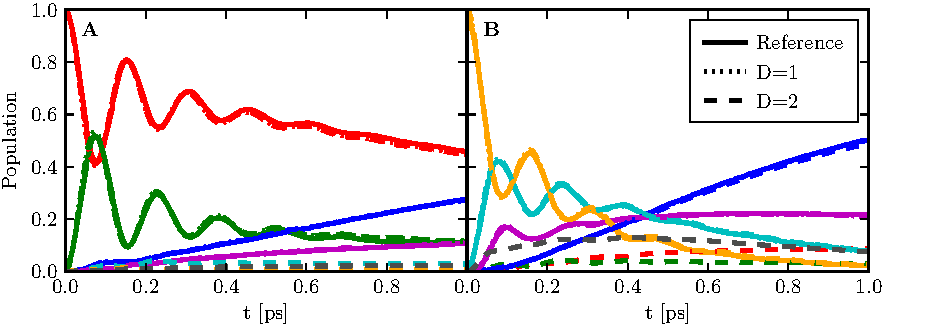
\includegraphics{img/fmo_ishfl}
  \caption{%
    Exciton transfer of the simplified FMO-monomer with seven BChls at 77\,K using the \NMSSE-hierarchy up to first~(dotted) and second order~(dashed) averaged over 10000 trajectories.
    For comparison, the solid line shows the reference results of Ishizaki and Fleming~\cite{IsFl09_fmo}, which were obtained in the \HEOM approach.
    We show the population for BChls 1--4 \textbf{(A)} and BChls 3--6 \textbf{(B)} with initial excitation on site 1 and 6 respectively (see \autoref{fig:app.monomer_full} for the color code).
    The inset displays a purely electronic system without coupling to the vibrational degrees of freedom.
    Details on parameters can be found in \autoref{sec:tla.parameters}.
    \label{fig:app.fmo_ishfl}
  }

  \vspace{.3cm}
  \centering
  \begin{subfigure}[b]{0.3\textwidth}
    \includegraphics[width=\textwidth]{img/fmo_transfer_0.png}
    \caption{%
      $t = 0.00 \, \mathrm{ps}$
    }
  \end{subfigure}
  \begin{subfigure}[b]{0.3\textwidth}
    \includegraphics[width=\textwidth]{img/fmo_transfer_1.png}
    \caption{%
      $t = 0.2 \, \mathrm{ps}$
    }
  \end{subfigure}
  \begin{subfigure}[b]{0.3\textwidth}
    \includegraphics[width=\textwidth]{img/fmo_transfer_2.png}
    \caption{%
      $t = 0.50 \, \mathrm{ps}$
    }
  \end{subfigure}

  \begin{subfigure}[b]{0.3\textwidth}
    \includegraphics[width=\textwidth]{img/fmo_transfer_3.png}
    \caption{%
      $t = 1.00 \, \mathrm{ps}$
    }
  \end{subfigure}
  \begin{subfigure}[b]{0.3\textwidth}
    \includegraphics[width=\textwidth]{img/fmo_transfer_4.png}
    \caption{%
      $t = 2.00 \, \mathrm{ps}$
    }
  \end{subfigure}

  \caption{%
    Same as \autoref{fig:app.fmo_ishfl} B.
    The intensity of each molecule represents the population of the associated exciton state.
    For the sake of clarity we do not show the full molecular structure.
    \label{fig:app.fmo_transport_pretty}
  }
\end{figure}
%%%%%%%%%%%%%%%%%%%%%%%%%%%%%%%%%%%%%%%%%%%%%%%%%%%%%%%%%%%%%%%%%%%%%%%%%%%%%%%%

\Autoref{fig:app.fmo_ishfl} shows the results of our calculations at cryogenic temperature $T=77\,\mathrm{K}$ using pure state hierarchy as well as the established \HEOM-results of Ishizaki and Fleming \cite{IsFl09_fmo}.
Both initial excitations move remarkably fast and directed---and up to $t=700\,\mathrm{fs}$ in a quantum-coherent, wavelike fashion---toward the energy sink at BChl 3.
However, the final population of the latter is only about half as large on the left hand side due to the relatively high site energy of BChl 2.
This prolongs the lifetime of an exciton-state on BChl 1 significantly, or, put differently, the electronic excitation remains on the first site for a long time.

It was conjectured that this barrier is partly responsible for the high yield of the FMO-complex \cite{IsFl09_fmo}.
Indeed, the relatively small energy gap $\Delta\epsilon = 200\, \mathrm{cm^{-1}}$ between the first and third BChl is overcome quite easily by virtue of thermal excitation leading to a loss of population on the third site through this channel.
The larger gap of $\Delta\epsilon = 300\,\mathrm{cm^{-1}}$ between the second and the third molecule suppresses depopulation much more efficiently.
This is exactly where quantum effects influence the operation significantly:
The subsidiary energetic minima at BChl 1, which would practically trap a classical-hopping excitation, is overcome much quicker due to quantum-mechanical delocalization.

No such initial \quotes{energy barrier} exists for the transport starting at BChl 6, therefore, the yield at BChls 3 and 4 is almost three-quarters of the total population at $t=1\,\mathrm{ps}$.
For even longer times, all other sites show almost complete depopulation as shown in \autoref{fig:app.fmo_transport_pretty}.

In the inset to \autoref{fig:app.fmo_ishfl} we also show the dynamics for a purely electronic system:
As expected, the population shows a purely oscillatory behavior with no effective excitation transport, thus emphasizing the importance of vibrational degrees of freedom in the exciton energy transfer.\\

Remarkably, the results of first and second order in the \NMSSE-hierarchy are almost indistinguishable from each other and agree very well with the reference.
Calculations including one more order (not shown) verify that the second order is already enough to obtain convergence in these parameter regimes.
As we show in \autoref{sec:tla.parameters}, the inverse correlation time\footnote{%
  Recall our notation $\alpha(t) = g \, \exp[-\gamma t]$ for $t > 0$.
}
of the dominant mode is given by $\gamma = 106\,\mathrm{cm^{-1}}$.
Therefore, the proposed truncation condition~\ref{eq:num.truncation_condtion}, namely $\omega_\mathrm{sys} \ll D \gamma$, with the typical system frequency $\omega_\mathrm{sys} \approx 500\,\ucm^{-1}$ is too restricting, yet.
This strengthens the statement that convergence with respect to truncation order should be checked individually for each set of parameters.

%% Spectral density and bcf plot  %%%%%%%%%%%%%%%%%%%%%%%%%%%%%%%%%%%%%%%%%%%%%%
  \begin{figure}
    \centering
    \includegraphics[width=\columnwidth]{img/fmo_bcf}
    \caption{%
      Environmental parameters used for the FMO-complex.
      \textbf{(A)} Drude spectral density with reorganization energy $\lambda = 35\,\mathrm{cm^{-1}}$, and relaxation time $\gamma^{-1} = 50\,\mathrm{fs}$.
      \textbf{(B)} Bath correlation function at 77\,K and 300\,K.
      The imaginary part with (dotted) and without (dashed) almost-Markovian correction is identical for both (for details see \autoref{tb:fmo.bcfs}).
    }
    \label{fig:app.fmo_bcf}
  \end{figure}
%%%%%%%%%%%%%%%%%%%%%%%%%%%%%%%%%%%%%%%%%%%%%%%%%%%%%%%%%%%%%%%%%%%%%%%%%%%%%%%%

Nevertheless, we do not obtain complete agreement with the reference in \autoref{fig:app.fmo_ishfl} A for the reason discussed at the end of \autoref{sec:num.expansion}.
As shown in the appendix, the bath correlation function of a Drude spectral density always has a discontinuous jump in its imaginary part at the origin.
This manifests in the complex prefactor $g$ of the exponential mode, which cannot be adjusted by the low-temperature correction term as the dashed line in \autoref{fig:app.fmo_bcf} B indicates.
But since $\alpha(t)$ is related to our driving processes $\ZZ_t$ by $\alpha(t-s) = \E[Z_t \ZZ_s]$, we cannot reproduce such a correlation function in the driving noise.
However, we approximate the discontinuous jump by including an additional, almost-Markovian mode with purely imaginary $g$, such that $\Im\alpha(t)$ goes smoothly to zero as $t \to 0$ while changing $\alpha$ as little as possible---the result is indicated by a dotted line in \autoref{fig:app.fmo_bcf} B.
Since the low-temperature correction mode is already approximated with an almost-Markovian mode, this does not increase the computational expense.\\


%% MevsPhi plot %%%%%%%%%%%%%%%%%%%%%%%%%%%%%%%%%%%%%%%%%%%%%%%%%%%%%%%%%%%%%%%%
\begin{figure}[p]
  \centering
  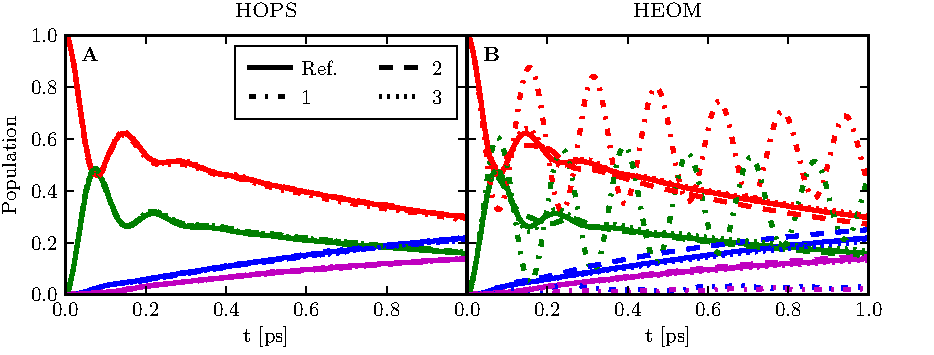
\includegraphics[width=\columnwidth]{img/fmo_mevsphi}
  \caption{%
    Exciton transfer of the simplified FMO-monomer at 300\,K for BChls 1--4 with initial excitation on site 1 and internal convergence check of the hierarchies.
    Solid lines display the reference results \cite{IsFl09_fmo}.\\
    \textbf{(A)} \NMSSE-hierarchy with 10000 realizations and truncation orders 1--3.\\
    \textbf{(B)} Same sets of parameters, but calculated in the \HEOM formalism with truncation at orders 1, 3 and 5 using \textsc{PHI} \cite{StSc12_heom}.\\
    \textbf{(C)} The deviation of the stochastic hierarchy with respect to its third order result. Dotted lines indicate the maximum value over time. The starred curves correspond to a larger sample size of 50000 realizations.\\
    \textbf{(D)} Same as (C), but for the \HEOM calculation. Here, the reference is the fifth order result.
  }
  \label{fig:app.fmo_mevsphi}
\end{figure}
%%%%%%%%%%%%%%%%%%%%%%%%%%%%%%%%%%%%%%%%%%%%%%%%%%%%%%%%%%%%%%%%%%%%%%%%%%%%%%%%

The exciton dynamics at physiological temperature in \autoref{fig:app.fmo_mevsphi} shows a similar qualitative behavior.
However, the transfer is less efficient and directed, as decoherence leads to a much stronger smearing of the excitation over all BChls, even the ones not shown in this picture.
For the same reason, the wave-like motion only lasts up to $t \approx 400\,\mathrm{fs}$.
Notwithstanding, at $t = 1\,\mathrm{ps}$ the population of the relevant, third BChl is $0.2$---still about two-thirds of the result at cryogenic temperature---and increases further.

This time, the \NMSSE-hierarchical equations of motion reproduce the results of Ishizaki-Fleming almost exactly and once again, differences between first, second and third order are negligible.
We see in \autoref{fig:app.fmo_bcf} that the imaginary part of $\alpha(0)$ is now very small compared to its real part, therefore, the deviations it caused at $77\,\mathrm{K}$ are not relevant at higher temperatures.
Nevertheless, the differences between first and second order are more pronounced than in the low temperature calculations.
Of course, this is due to the larger real-part of the coupling constant $\Re\alpha(0) = \Re g=14279\,\mathrm{cm^{-1}}$ compared to $\Re g=2916\,\ucm^{-1}$ for $T=77\,\mathrm{K}$, as discussed in \autoref{sub:num.spin_boson.depth}.
The second, almost-Markovian mode is irrelevant for the truncation due to its large inverse correlation-time $\gamma = 1000\,\ucm^{-1}$.

On the right hand side of \autoref{fig:app.fmo_mevsphi} B, we carry out the same calculations in the \HEOM-formalism \cite{StSc12_heom}.
Clearly, for a good approximation we need a much larger truncation order.
The first order calculation displays highly undamped oscillations and further auxiliary states are necessary to get the qualitative picture right.
We have found that a truncation at fifth order is necessary to correctly reproduce the coherent oscillations between 0\,fs and 300\,fs.

To check internal convergence of each method systematically, we proceed as follows:
First we define a measure for deviation of a given reduced density matrix $\rho(t) = \rho_D(t)$, obtained from a numerical calculation up to order $D$, with respect to some reference $\rho^{\mathrm{ref}}(t)$ as
\begin{equation}
  A[\rho(t), \rho^\mathrm{ref}(t)] = \max\limits_n \left\vert \rho_{nn}(t) - \rho^{\mathrm{ref}}_{nn}(t) \right\vert.
  \label{eq:app.accuracy}
\end{equation}
Since we confine our discussion to the population of the exciton states $n$ given by $\rho_{nn}$, $A$ reflects the deviations seen in the pictures.
Also, we are only interested in the convergence of the density matrix or pure state hierarchy itself, therefore, the reference state $\rho^\mathrm{ref} = \rho_D$ is calculated  with the same method and selected by increasing the truncation order $D$ until $A[\rho_{D-1}(t), \rho_{D}(t)] \approx 10^{-2}$.
This amounts to $D=3$ for the \NMSSE-hierarchy and $D=5$ for the $\HEOM$-formalism.
The accuracy of lower-order calculations with respect to the chosen reference is shown in \autoref{fig:app.fmo_mevsphi} C and D for the \NMSSE and the density matrix hierarchy, respectively.

We already mentioned in the general discussion above that within the pure state hierarchy, the first order's deviation from the third order of about 2\% is barely visible in \autoref{fig:app.fmo_mevsphi} A.
In contrast, the same accuracy is obtained in the \HEOM-formalism not until we truncate the hierarchy at third order (neglecting even stronger deviations for $t < 300\,\mathrm{fs}$).
But there is a major difference between the two approaches:
The \HEOM-calculations show the largest discrepancy at the initial wave-like motion and then the accuracy improves by about an order of magnitude, whereas the deviations of the \NMSSE-hierarchy remain more or less constant  after $t = 0.2\,\mathrm{ps}$ for the first order or oscillate irregularly for the second order calculations.
These observations indicate that at this level of accuracy the errors of the Monte-Carlo sampling play a significant role.
We check this statement by repeating the same calculations using a larger sample size---a star marks the corresponding results in \autoref{fig:app.fmo_mevsphi}.
The slightly better accuracy supports this statement, but a clear confirmation would require a tremendous number of realizations.\\



In conclusion, the discussion above shows that the hierarchical equations based on the nonlinear \NMSSE provide a highly efficient method to calculate exciton energy transfer dynamics in the FMO-complex.
We obtain almost perfect agreement for both, 77\,K and 300\,K, with the established results of Ishizaki and Fleming in first order calculations.
The discrepancy of these to higher order calculations is less than a few percent, demonstrating very rapid convergence with respect to the truncation order.
Of course, the achieved accuracy is completely unnecessary for most investigations on biological systems, because the theoretical model itself is usually much less reliable due to approximations and experimental errors for the parameters involved.
Also, the improved numerical efficiency, due to a reduced number of auxiliary states\footnote{%
  In the case of a single bath mode, we have eight auxiliary states for $D=1$ compared to 330 for $D=4$.
}
and propagating Hilbert space vectors instead of density matrices, is more than compensated by the large sample size required.
However, the stochastic hierarchies' advantages really come to fruition when dealing with more complex systems.
For example, data from fluorescence line-narrowing measurements on \emph{Prosthecochloris aesturaii} indicate \cite{AdRe06_fmo} that more realistic spectral densities are far more structured, requiring about 25 exponential modes\footnote{%
  The spectral density of Fig.~2 in the cited reference can be approximately described with 12 anti-symmetrized Lorentzians, each amounting to two exponential modes.
  Additional correction terms are necessary depending on the temperature.
}.
This amounts to 176 auxiliary states for $D=1$ compared to a tremendous number of 41 million states required by a fourth-order calculation.
Although it is not clear, if such a low-order truncation still produces accurate results for more structured environments, the improved convergence compared to the \HEOM-formalism might be crucial for the treatment of more realistic systems.


%%%%%%%%%%%%%%%%%%%%%%%%%%%%%%%%%%%%%%%%%%%%%%%%%%%%%%%%%%%%%%%%%%%%%%%%%%%%%%%%
\section{Absorption Spectra of Molecular Aggregates}
\label{sec:app.spectra}
% * experimental setup
% * why not so good, but we still use them -> 2D spectroscopy
%%%%%%%%%%%%%%%%%%%%%%%%%%%%%%%%%%%%%%%%%%%%%%%%%%%%%%%%%%%%%%%%%%%%%%%%%%%%%%%%

The second exemplary application of our pure-state hierarchy is the calculation of absorption spectra in molecular aggregates.
In general, the \NMSSE provides a highly efficient framework to attack this problem, since all the relevant information is encoded in a single realization $\psi_t(\ZZ = 0)$ and no stochastic average is necessary.
In a previous work based on the convolutionless formulation~\ref{eq:nmqsd.nmsse_o} in ZOFE approximation, good agreement with the exact pseudo-mode approach\footnote{%
  The pseudo-mode approach amounts to replacing exponential modes of the bath correlation function by a harmonic oscillator coupled to a Markovian environment \cite{Imot94_}.Although formally exact, this approach is quite limited in application due to large computational demands.
}
was achieved in large parts of the parameter space \cite{RoStEi11_nmqsd_aggregats}.
However, for intermediate values of the electronic coupling $V_{mn}$ noticeable deviations occurred.
Here, we show that the linear hierarchy~\ref{eq:num.hierarchy_lin} is equally well suited for this task, but with the additional benefit that a systematic improvement is achieved by increasing the truncation order.


%%%%%%%%%%%%%%%%%%%%%%%%%%%%%%%%%%%%%%%%%%%%%%%%%%%%%%%%%%%%%%%%%%%%%%%%%%%%%%%%
\subsection{NMSSE for Spectra}
\label{sub:app.spectra.nmsse}
% * why nmsse so good for this?

In this section, we demonstrate the simple connection between solutions of the linear \NMSSE with $\ZZ_t = 0$ and absorption spectra of molecular aggregate at zero temperature \cite{RoEiWo09_aggregats,RoStEi11_nmqsd_aggregats}.
Using the thermo-field construction from \autoref{sec:nmqsd.temperature}, we can treat an arbitrary thermal environment along the same lines \cite{RiStEi13_prep}.
Clearly, for $T = 0\,\mathrm{K}$ the initial state of the aggregate is given by $\ket{0_\mathrm{el}}\otimes\ket{0}$ with the electronic ground state $\ket{0_\mathrm{el}}$ defined in \autoref{eq:app.ground_state} and the vibrational ground state $\ket{0}$.
In dipole-approximation, the absorption coefficient of light with frequency $\nu$ and polarization $\rvec{E}$ is given by \cite{MaKu11_dynamics}
\begin{equation}
  A(\nu) = \Re \left( \int_0^\infty \exp[\ii\nu t] M(t) \dd t \right),
  \label{eq:app.absorption}
\end{equation}
where the dipole-correlation function reads
\begin{equation}
  M(t) = \bra{0_\mathrm{el}}\bra{0} \rvec\mu\cdot\rvec{E} \, \exp[-\ii \opH{agg} t] \, \rvec\mu\cdot\cc{\rvec{E}} \ket{0_\mathrm{el}}\ket{0}.
  \label{eq:app.dipole_correlation}
\end{equation}
Here, $\rvec\mu = \sum_m \rvec\mu_m$ denotes the total dipole operator of the aggregate and $\opH{agg} = \opH{el}^{(0)} + \opH{el}^{(1)} + \Henv$ is the total aggregate Hamiltonian restricted to the electronic subspace with at most one exciton.
Provided the dipole-operators are independent of the vibrational degrees of freedom, inserting complete sets of electronic basis vectors $\sum_m \ket{m}\bra{m}$ in \autoref{eq:app.dipole_correlation} yields
\begin{equation}
  M(t) = \sum_{m,n} \cc{d}_m d_n \, \bra{m}\bra{0} \exp[-\ii \opH{agg} t] \ket{n} \ket{0}
  \label{eq:app.dipole_correlation_two}
\end{equation}
with the transition dipole-elements projected in the direction of polarization
\begin{equation*}
  d_m = \bra{m} \rvec\mu \cdot \cc{\rvec{E}} \ket{0_\mathrm{el}}.
\end{equation*}
Since the expectation value of the time evolution operator in \autoref{eq:app.dipole_correlation_two} includes only contributions from the one-exciton subspace, it is equivalent to
\begin{equation*}
  M(t) = \left(\sum_m \cc{d}_m \bra{m}\bra{0} \right) \exp[-\ii \opH{agg}^{(1)} t] \left(\sum_n d_n \ket{n}\ket{0} \right) = \abs{\vec{d}}^2 \braket{\Psi_0}{\Psi_t}.
\end{equation*}
with $\opH{agg}^{(1)} = \opH{el}^{(1)} + \Henv$ given by \autoref{eq:app.agg_hamil_twolevel}
Here, $\ket{\Psi_t}$ denotes the solution to
\begin{equation}
  \partial_t \ket{\Psi_t} = -\ii \opH{agg}^{(1)} \ket{\Psi_t}, \qquad \ket{\Psi_0} = \ket{\psi_0}\otimes\ket{0}
  \label{eq:app.eqom}
\end{equation}
with the initial electronic state $\ket{\psi_0} = \abs{\vec d}^{-1} \, \sum_m d_m \ket{m}$.
The sum of the dipole-elements $\abs{\vec{d}}^2 = \sum_n \abs{d_n}^2$ is introduced to ensure normalization of $\ket{\psi_0}$.\\



\Autoref{eq:app.eqom} is already very close to the microscopic version of our {\NMSSE}.
The only difference to \autoref{eq:nmqsd.hamiltonian_microsopic} is that the latter is formulated in the interaction picture.
However, transforming the time evolution picture leaves the scalar product $\braket{\Psi_0}{\Psi_t}$ and the initial state $\ket{\Psi_0} = \ket{\psi_0} \otimes \ket{0}$ unchanged.
Therefore, we can insert the resolution of unity for coherent states~\ref{eq:nmqsd.identity} and obtain
\begin{equation*}
  M(t) = \abs{\vec d}^2 \int \frac{\mathrm{d}^{2N}z}{\pi^N} \, \braket{\psi_0}{\psitz} \, \braket{0}{\zz},
\end{equation*}
where $\psitz$ is the solution to \autoref{eq:nmqsd.hamiltonian_microsopic}.
As $\braket{0}{\zz} = 1$ and $\braket{\psi_0}{\psi_t(\cc\zz)}$ is analytical in $\cc\zz$, the only term of the corresponding Taylor series that is not canceled by the integral is independent of $\cc\zz$.
In other words, the dipole correlation function expressed in terms of solutions $\psitZ$ of the linear \NMSSE reads
\begin{equation}
  M(t) = \abs{\vec d}^2 \, \braket{\psi_0}{\psi_t(\cc\zz = 0)} = \abs{\vec d}^2 \, \braket{\psi_0}{\psi_t(\ZZ = 0)}.
  \label{eq:app.dipole_correlation_nmsse}
\end{equation}
Of course, this does not imply that we can simply neglect the functional derivative in the {\NMSSE}.
Nevertheless, the corresponding hierarchy~\ref{eq:num.hierarchy_lin} is completely local in $\ZZ_t$, so we can set $\ZZ_t = 0$ in each order.
In conclusion, assuming a single exponential bath mode $\alpha(t) = g\,\exp[-(\gamma + \ii\Omega) t]$ ($t > 0$), the relevant trajectory $\psi_t(\ZZ = 0) =: \psit[0]$ satisfies the following set of equations
\begin{equation}
  \partial_t\psit[k] = (-\ii\Hsys -  k(\gamma + \ii\Omega)\psit[k] + k \alpha(0) \psit[k-1] - \adj{L} \psit[k+1],
  \label{eq:app.spectrum_hierarchy}
\end{equation}
with initial conditions $\psi_0^{(0)} = \psi_0$ and $\psi_0^{(k)} = 0$ ($k \ge 1$).

%%%%%%%%%%%%%%%%%%%%%%%%%%%%%%%%%%%%%%%%%%%%%%%%%%%%%%%%%%%%%%%%%%%%%%%%%%%%%%%%
\subsection{Results}
\label{sub:app.spectra.results}
% * other techniques
% * cool behavior of hierarchies

%% Spectra plot %%%%%%%%%%%%%%%%%%%%%%%%%%%%%%%%%%%%%%%%%%%%%%%%%%%%%%%%%%%%%%%%
\begin{figure}[p]
  \centering
  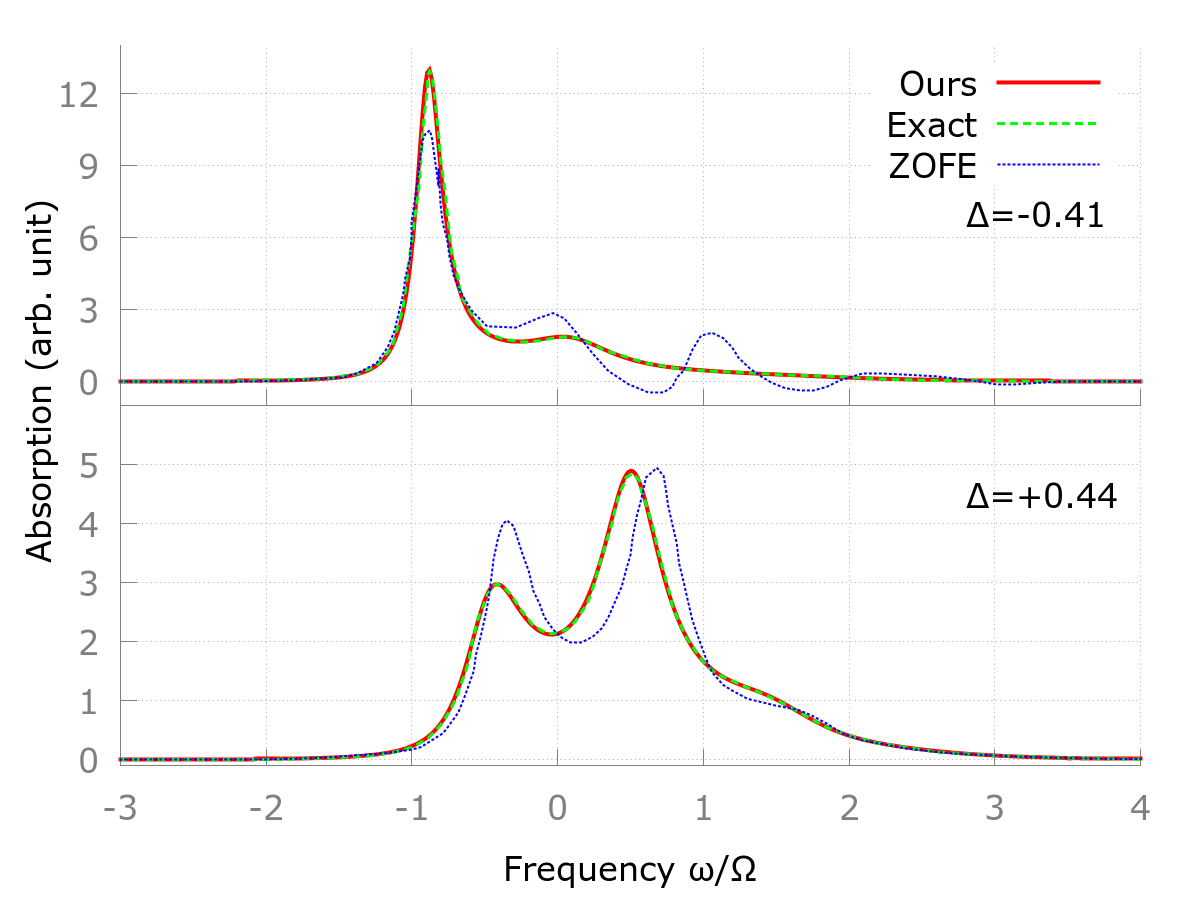
\includegraphics[width=\columnwidth]{img/spectra}
  \caption{%
    Absorption spectra of a dimer and a single-mode bath correlation function with $g = 0.64\,\Omega$, $\gamma=0.1\,\Omega$ (left) and $\gamma=0.25\,\Omega$ (right).
    The \NMSSE-hierarchy results (blue) with truncation at first (solid), third (dotted) and fifth (dashed) order are compared to the pseudo-mode spectra (red).
  }
  \label{fig:app.spectra}
\end{figure}
%%%%%%%%%%%%%%%%%%%%%%%%%%%%%%%%%%%%%%%%%%%%%%%%%%%%%%%%%%%%%%%%%%%%%%%%%%%%%%%%

As a demonstration, we investigate absorption spectra of linear aggregates with identical monomers and parallel dipole-moments in this section.
For the electronic interaction we assume nearest-neighbor coupling with equal strength, that is $V_{mn} = (V\delta_{m,n+1} + V\delta_{m, n-1})$.
The vibrational degrees of freedom are described by a single exponential mode $\alpha(t) = \exp[-\gamma\abs{t} - \ii\Omega t]$.
We use the results of Roden, Strunz and Eisfeld \cite{RoStEi11_nmqsd_aggregats} obtained in the exact pseuo-mode approach as a reference, but also compare a few aspects to the \textsc{ZOFE}-results from the same work.

\Autoref{fig:app.spectra} displays the spectra of a dimer for two widths of the spectral density, namely $\gamma=0.25\,\Omega$ and $\gamma=0.1\,\Omega$, and different coupling strengths $V$.
Using the truncation order $D = 5$ (dashed line), we obtain perfect agreement with the reference for all values of $V$.
To investigate the behavior for smaller truncation orders, we also show the results for $D=1$ (solid) and $D=3$ (dotted).
Not surprising, these approximate the exact result better in the case of larger $\gamma=0.25$ compared to $\gamma=0.1$.
Similar to the \textsc{ZOFE}-approach, best agreement is achieved for large values of $\abs{V}$, because the impact of the environment is reduced by a strong electronic Hamiltonian.
For smaller $\abs{V}$, the influence of the environment grows and more auxiliary states are needed in order to reproduce the reference's results.
However, while \textsc{ZOFE} is exact for $V = 0$ \cite{RoStEi11_nmqsd_aggregats}, the first order \NMSSE-hierarchy shows about the same amount of deviation as in the $V=-0.41$ plot.


Remarkably, the \NMSSE-hierarchy improves systematically with increasing truncation order.
Already the first order calculations reproduce the position of the lowest energy peak---and for $V < 0$ the magnitude as well---with very high precision.
This behavior continues for the next peaks, too, as the spectra for $V=0.44$ show:
Although the higher-frequency spectrum $\nu > 0$ is obtained correctly only for the maximum truncation order $D = 5$, the position of the second peak is well-approximated at the intermediate value $D = 3$.

%%%%%%%%%%%%%%%%%%%%%%%%%%%%%%%%%%%%%%%%%%%%%%%%%%%%%%%%%%%%%%%%%%%%%%%%%%%%%%%%
\begin{figure}[t]
  \centering
  \includegraphics[width=\columnwidth]{img/ptcda}
  \caption{%
    Absorption spectrum for the \textsc{PTCDA}-dimer convoluted with a Gaussian of width $\sigma = 20\,\mathrm{cm^{-1}}$ with electronic coupling $V=600\,\mathrm{cm^{-1}}$ and different truncation orders $D$ of the hierarchy.
    The black lines display the sharp peaks of the spectrum for $D=7$ with a much narrower enveloping Gaussian ($\sigma = 1\,\mathrm{cm^{-1}}$).
    We use a bath correlation function with six purely-oscillatory exponentials, see \autoref{tb:tla.spectra} for the parameters \cite[Tab.\,1 D]{RoEiDv11_ptcda}.
  }
  \label{fig:app.ptcda}
\end{figure}
%%%%%%%%%%%%%%%%%%%%%%%%%%%%%%%%%%%%%%%%%%%%%%%%%%%%%%%%%%%%%%%%%%%%%%%%%%%%%%%%

To strengthen this statement, we study a more complex system, namely a \textsc{PTCDA} dimer with a bath correlation function consisting of six exponential modes.
The latter was already used as an approximation to a realistic environment in pseudo-mode calculations \cite{RoEiDv11_ptcda}.
In contrast to the rest of this work, all modes under consideration are purely oscillatory, that is $\gamma = 0$.
Nevertheless, \autoref{fig:app.ptcda} clearly shows a behavior similar to the previous spectra~\ref{fig:app.spectra} with increasing truncation order $D$:
Even the first order $D=1$ yields the correct position of the lowest major peak at wavenumber $k \approx -800\,\ucm^{-1}$ with good precision, but fails at higher energies.
The next order shown ($D=3$) roughly reproduces the correct magnitude and position for the three characteristic peaks on the left and approximately indicates the smaller structure between the two major peaks at $k \approx -800\,\ucm^{-1}$ and $k \approx 700\,\ucm^{-1}$.
The latter marks the upper boundary for the region where the two highest order calculations with $D=5$ and $D=7$ practically coincide.
For even higher wavenumber, deviations are pronouncedly visible but not random.
Roughly, the highest order calculation only improves the position and magnitude of the peaks that are already present for $D=5$.\\



Summarizing the above, we have demonstrated that the hierarchy of pure states provides an efficient tool to study absorption spectra of quantum aggregates.
In contrast to the study of the time evolution of a reduced density matrix, the calculation of spectra in the \NMSSE-formalism requires no Monte-Carlo average over several realizations.
Therefore, one major advantage of the \NMSSE compared to density-matrix formalisms, namely the propagation of state vectors, really comes into its own.
This combined with the very predictable behavior for a growing number of hierarchy orders allows studying large-dimensional systems coupled to a highly structured environment, especially the low-energy part of the spectra.
Besides, we have also demonstrated that truncation of the \NMSSE-hierarchy is possible for $\gamma \to 0$, exemplifying applicability of this approach even in the highly non-Markovian limit.
